% Created 2014-10-23 jue 12:56
\documentclass[xcolor={usenames,svgnames,dvipsnames}]{beamer}
\usepackage[utf8]{inputenc}
\usepackage[T1]{fontenc}
\usepackage{fixltx2e}
\usepackage{graphicx}
\usepackage{longtable}
\usepackage{float}
\usepackage{wrapfig}
\usepackage{rotating}
\usepackage[normalem]{ulem}
\usepackage{amsmath}
\usepackage{textcomp}
\usepackage{marvosym}
\usepackage{wasysym}
\usepackage{amssymb}
\usepackage{hyperref}
\tolerance=1000
\usepackage{color}
\usepackage{listings}
\AtBeginSubsection[]{\begin{frame}[plain]\tableofcontents[currentsubsection,sectionstyle=show/shaded,subsectionstyle=show/shaded/hide]\end{frame}}
\lstset{keywordstyle=\color{blue}, commentstyle=\color{gray!90}, basicstyle=\ttfamily\small, columns=fullflexible, breaklines=true,linewidth=\textwidth, backgroundcolor=\color{gray!23}, basewidth={0.5em,0.4em}, literate={á}{{\'a}}1 {ñ}{{\~n}}1 {é}{{\'e}}1 {ó}{{\'o}}1 {º}{{\textordmasculine}}1}
\usepackage{mathpazo}
\hypersetup{colorlinks=true, linkcolor=Blue, urlcolor=Blue}
\usepackage{fancyvrb}
\DefineVerbatimEnvironment{verbatim}{Verbatim}{boxwidth=\textwidth, fontsize=\tiny, formatcom = {\color{black!70}}}
\usepackage{animate}
\usetheme{Goettingen}
\usecolortheme{rose}
\usefonttheme{serif}
\author{Oscar Perpiñán Lamigueiro}
\date{24 de Octubre de 2014}
\title{Visualización de Series Temporales}
\hypersetup{
  pdfkeywords={},
  pdfsubject={},
  pdfcreator={Emacs 24.3.1 (Org mode 8.2.7c)}}
\begin{document}

\maketitle

\section{Introducción}
\label{sec-1}

\subsection{Paquetes}
\label{sec-1-1}
\begin{frame}[label=sec-1-1-1]{CRAN Task View}
\begin{block}{\href{http://CRAN.R-project.org/view\%3DTimeSeries}{CRAN Tasks View ``Time Series Analysis'''}}
\begin{itemize}
\item \href{http://cran.r-project.org/web/packages/zoo/vignettes/zoo.pdf}{zoo}
\item \href{http://cran.r-project.org/web/packages/xts/vignettes/xts.pdf}{xts}
\end{itemize}
\end{block}
\begin{block}{Referencias}
\begin{itemize}
\item Ripley y Hornik, 2001. \href{http://CRAN.R-project.org/doc/Rnews/Rnews_2001-2.pdf}{Date Time Classes}
\item Grothendieck y Petzoldt, 2004. \href{http://CRAN.R-project.org/doc/Rnews/Rnews_2004-1.pdf}{Date and Time Classes in R}
\end{itemize}
\end{block}
\end{frame}

\begin{frame}[fragile,label=sec-1-1-2]{zoo}
 \begin{itemize}
\item El paquete \texttt{zoo} define una clase \texttt{S3} y métodos para series temporales.
\item Los objetos \texttt{zoo} se crean con la función homónima:
\begin{itemize}
\item Los datos pueden ser un vector, una matriz, o un \texttt{factor} totalmente ordenados por un vector índice.
\item Este índice puede ser una medida de tiempo, pero no es imprescindible.
\end{itemize}
\item Define dos nuevos índices temporales: \texttt{yearmon} y \texttt{yearqtr}.
\item Incluye métodos asociados a funciones genéricas (\texttt{print}, \texttt{summary},
etc.) y a operaciones matemáticas.
\end{itemize}
\end{frame}
\begin{frame}[fragile,label=sec-1-1-3]{zoo: funciones básicas}
 \begin{itemize}
\item \texttt{coredata} extrae el contenido de un \texttt{zoo} (sin índice temporal).
\item \texttt{index} extrae el índice temporal.
\item \texttt{window} extrae una ventana temporal de un \texttt{zoo}.
\item \texttt{merge} y \texttt{cbind} unen dos \texttt{zoo} teniendo en cuenta los índices temporales.
\item \texttt{aggregate} parte un \texttt{zoo} en grupos definidos por alguna condición
sobre su índice temporal, calcula una función sobre cada grupo, y
devuelve la serie temporal agregada.
\end{itemize}
\end{frame}

\begin{frame}[fragile,label=sec-1-1-4]{zoo: funciones básicas}
 \begin{itemize}
\item \texttt{NA}: \texttt{na.omit}, \texttt{na.contiguous}, \texttt{na.approx}, \texttt{na.locf}.

\item \href{http://cran.r-project.org/web/packages/zoo/vignettes/zoo-read.pdf}{Escritura y lectura de datos}: \texttt{write.zoo} y \texttt{read.zoo}.
\end{itemize}
\end{frame}

\begin{frame}[fragile,label=sec-1-1-5]{xts}
 \begin{itemize}
\item \texttt{xts} amplia las funcionalidades de \texttt{zoo} implementando la notación
\href{http://en.wikipedia.org/wiki/ISO_8601}{ISO:8601} para extraer subconjuntos de una serie temporal.
\item Funciones importantes:
\begin{itemize}
\item \texttt{endpoints} identifica los puntos en los que termina una condición.
\item \texttt{to.period} cambia la periodicidad de una serie temporal.
\item \texttt{period.*} y \texttt{apply.*} evaluan una función sobre un conjunto de
periodos temporales.
\end{itemize}
\end{itemize}
\end{frame}

\subsection{Configuración}
\label{sec-1-2}
\begin{frame}[fragile,label=sec-1-2-1]{Cargar en el orden correcto}
 \lstset{language=R,label= ,caption= ,numbers=none}
\begin{lstlisting}
  library(lattice)
  library(ggplot2)
  library(latticeExtra)
  library(zoo)
\end{lstlisting}
\end{frame}
\begin{frame}[fragile,label=sec-1-2-2]{Tema para \texttt{lattice}}
 \lstset{language=R,label= ,caption= ,numbers=none}
\begin{lstlisting}
  myTheme <- custom.theme.2(pch=19, cex=0.7,
                            region=rev(brewer.pal(9,
                                name = 'YlOrRd')),
                            symbol = brewer.pal(n=8,
                                name = "Dark2"))
  myTheme$strip.background$col='transparent'
  myTheme$strip.shingle$col='transparent'
  myTheme$strip.border$col='transparent'
\end{lstlisting}
\end{frame}

\begin{frame}[fragile,label=sec-1-2-3]{Escalas}
 \lstset{language=R,label= ,caption= ,numbers=none}
\begin{lstlisting}
  xscale.components.custom <- function(...){
      ans <- xscale.components.default(...)
      ans$top=FALSE
      ans}
  yscale.components.custom <- function(...){
      ans <- yscale.components.default(...)
      ans$right=FALSE
      ans}
\end{lstlisting}
\end{frame}

\begin{frame}[fragile,label=sec-1-2-4]{Establecemos opciones por defecto}
 \lstset{language=R,label= ,caption= ,numbers=none}
\begin{lstlisting}
  myArgs <- list(as.table=TRUE,
                 between=list(x=0.5, y=0.2),
                 xscale.components = xscale.components.custom,
                 yscale.components = yscale.components.custom)
  defaultArgs <- lattice.options()$default.args
  
  lattice.options(default.theme = myTheme,
                  default.args = modifyList(defaultArgs, myArgs))
\end{lstlisting}
\end{frame}


\section{Serie Temporal Multivariante con Diferente Escala}
\label{sec-2}

\subsection{Datos}
\label{sec-2-1}

\begin{frame}[fragile,label=sec-2-1-1]{Aranjuez}
 \lstset{language=R,label= ,caption= ,numbers=none}
\begin{lstlisting}
  library(zoo)
  load('data/aranjuez.RData')
\end{lstlisting}
\end{frame}

\subsection{Primera aproximación}
\label{sec-2-2}

\begin{frame}[fragile,label=sec-2-2-1]{lattice: \texttt{xyplot}}
 \lstset{language=R,label= ,caption= ,numbers=none}
\begin{lstlisting}
  ## The layout argument arranges panels in rows
  xyplot(aranjuez, layout=c(1, ncol(aranjuez)))
\end{lstlisting}
\end{frame}
\begin{frame}[label=sec-2-2-2]{}
\includegraphics[width=.9\linewidth]{figs/aranjuez.pdf}
\end{frame}

\begin{frame}[fragile,label=sec-2-2-3]{ggplot2: \texttt{autoplot}}
 \lstset{language=R,label= ,caption= ,numbers=none}
\begin{lstlisting}
  autoplot(aranjuez) + facet_free()
\end{lstlisting}
\end{frame}
\begin{frame}[label=sec-2-2-4]{}
\includegraphics[width=.9\linewidth]{figs/aranjuezGG.pdf}
\end{frame}

\subsection{Anotaciones}
\label{sec-2-3}

\begin{frame}[fragile,label=sec-2-3-1]{lattice: Función completa}
 \lstset{language=R,label= ,caption= ,numbers=none}
\begin{lstlisting}
  library(grid)
  library(latticeExtra)
  
  ## Auxiliary function to extract the year value of a POSIXct time
  ## index
  Year <- function(x)format(x, "%Y")
  
  xyplot(aranjuez, layout=c(1, ncol(aranjuez)),
         strip=FALSE,
         scales=list(y=list(cex=0.6, rot=0)),
         panel=function(x, y, ...){
           ## Alternation of years
           panel.xblocks(x, Year,
                         col = c("lightgray", "white"),
                         border = "darkgray")
           ## Values under the average highlighted with red regions
           panel.xblocks(x, y<mean(y, na.rm=TRUE),
                         col = "indianred1",
                         height=unit(0.1, 'npc'))
           ## Time series
           panel.lines(x, y, col='royalblue4', lwd=0.5, ...)
           ## Label of each time series
           panel.text(x[1], min(y, na.rm=TRUE),
                      names(aranjuez)[panel.number()],
                      cex=0.6, adj=c(0, 0), srt=90, ...)
           ## Triangles to point the maxima and minima 
           idxMax <- which.max(y)
           panel.points(x[idxMax], y[idxMax],
                        col='black', fill='lightblue', pch=24)
           idxMin <- which.min(y)
           panel.points(x[idxMin], y[idxMin],
                        col='black', fill='lightblue', pch=25)
         })
\end{lstlisting}
\end{frame}

\begin{frame}[fragile,label=sec-2-3-2]{lattice: \texttt{panel.xblocks}}
 \begin{itemize}
\item Paquetes y función auxiliar
\end{itemize}
\lstset{language=R,label= ,caption= ,numbers=none}
\begin{lstlisting}
  library(grid)
  library(latticeExtra)

  ## Auxiliary function to extract the year value of a POSIXct time
  ## index
  Year <- function(x)format(x, "%Y")
\end{lstlisting}

\lstset{language=R,label= ,caption= ,numbers=none}
\begin{lstlisting}
## Alternation of years
panel.xblocks(x, Year,
              col = c("lightgray", "white"),
              border = "darkgray")
## Values under the average highlighted with red regions
panel.xblocks(x, y<mean(y, na.rm=TRUE),
                         col = "indianred1",
              height=unit(0.1, 'npc'))
\end{lstlisting}
\end{frame}
\begin{frame}[fragile,label=sec-2-3-3]{lattice: \texttt{panel.lines}}
 \lstset{language=R,label= ,caption= ,numbers=none}
\begin{lstlisting}
           ## Time series
           panel.lines(x, y, col='royalblue4', lwd=0.5, ...)
\end{lstlisting}
\end{frame}

\begin{frame}[fragile,label=sec-2-3-4]{lattice: \texttt{panel.text}}
 \lstset{language=R,label= ,caption= ,numbers=none}
\begin{lstlisting}
           ## Label of each time series
           panel.text(x[1], min(y, na.rm=TRUE),
                      names(aranjuez)[panel.number()],
                      cex=0.6, adj=c(0, 0), srt=90, ...)
\end{lstlisting}
\end{frame}


\begin{frame}[fragile,label=sec-2-3-5]{lattice: \texttt{panel.points}}
 \lstset{language=R,label= ,caption= ,numbers=none}
\begin{lstlisting}
           ## Triangles to point the maxima and minima 
           idxMax <- which.max(y)
           panel.points(x[idxMax], y[idxMax],
                        col='black', fill='lightblue', pch=24)
           idxMin <- which.min(y)
           panel.points(x[idxMin], y[idxMin],
                        col='black', fill='lightblue', pch=25)
\end{lstlisting}
\end{frame}

\begin{frame}[label=sec-2-3-6]{}
\includegraphics[width=.9\linewidth]{figs/aranjuezXblocks.pdf}
\end{frame}

\begin{frame}[fragile,label=sec-2-3-7]{ggplot2: acomodamos datos}
 \begin{itemize}
\item ggplot2 necesita un \texttt{data.frame} en formato \emph{long}: \texttt{fortify}
\end{itemize}
\lstset{language=R,label= ,caption= ,numbers=none}
\begin{lstlisting}
  timeIdx <- index(aranjuez)
  
  long <- fortify(aranjuez, melt=TRUE)
\end{lstlisting}
\end{frame}
\begin{frame}[fragile,label=sec-2-3-8]{ggplot2}
 \begin{itemize}
\item Bandas de valores por debajo de la media
\end{itemize}
\lstset{language=R,label= ,caption= ,numbers=none}
\begin{lstlisting}
  ## Values below mean are negative after being centered
  scaled <- fortify(scale(aranjuez, scale=FALSE), melt=TRUE)
  ## The 'scaled' column is the result of the centering.
  ## The new 'Value' column store the original values.
  scaled <- transform(scaled, scaled=Value,
                      Value=long$Value)
  underIdx <- which(scaled$scaled <= 0)
  ## 'under' is the subset of values below the average
  under <- scaled[underIdx,]
\end{lstlisting}
\end{frame}

\begin{frame}[fragile,label=sec-2-3-9]{ggplot2}
 \begin{itemize}
\item Bandas consecutivas de años: \texttt{xts::endpoints}
\end{itemize}

\lstset{language=R,label= ,caption= ,numbers=none}
\begin{lstlisting}
  library(xts)
  ep <- endpoints(timeIdx, on='years')
  N <- length(ep[-1])
  ## 'tsp' is start and 'tep' is the end of each band
  tep <- timeIdx[ep]
  tsp <- timeIdx[ep[-(N+1)]+1]
  ## 'cols' is a vector with the color of each band
  cols <- rep_len(c('gray', 'white'), N)
\end{lstlisting}
\end{frame}
\begin{frame}[fragile,label=sec-2-3-10]{ggplot2}
 \begin{itemize}
\item Mínimos y máximos.
\end{itemize}
\lstset{language=R,label= ,caption= ,numbers=none}
\begin{lstlisting}
  minIdx <- timeIdx[apply(aranjuez, 2, which.min)]
  minVals <- apply(aranjuez, 2, min, na.rm=TRUE)
  mins <- data.frame(Index=minIdx,
                     Value=minVals,
                     Series=names(aranjuez))
  
  maxIdx <- timeIdx[apply(aranjuez, 2, which.max)]
  maxVals <- apply(aranjuez, 2, max, na.rm=TRUE)
  maxs <- data.frame(Index=maxIdx,
                     Value=maxVals,
                     Series=names(aranjuez))
\end{lstlisting}
\end{frame}

\begin{frame}[fragile,label=sec-2-3-11]{ggplot2: resultado}
 \lstset{language=R,label= ,caption= ,numbers=none}
\begin{lstlisting}
  ggplot(data=long, aes(Index, Value)) +
      ## Time series of each variable
      geom_line(colour = "royalblue4", lwd = 0.5) +
      ## Year bands
      annotate(geom='rect', ymin = -Inf, ymax = Inf,
                xmin=tsp, xmax=tep,
                fill = cols, alpha = 0.4) +
      ## Values below average
      geom_rug(data=under,
               sides='b', col='indianred1') +
      ## Minima
      geom_point(data=mins, pch=25) +
      ## Maxima
      geom_point(data=maxs, pch=24) +
      ## Axis labels and theme definition
      labs(x='Time', y=NULL) +
      theme_bw() +
      ## Each series has different panel and y-scale
      facet_free()
\end{lstlisting}
\end{frame}


\section{Serie Temporal Multivariante con Misma Escala}
\label{sec-3}

\subsection{Primera aproximación}
\label{sec-3-1}
\begin{frame}[fragile,label=sec-3-1-1]{Datos}
 \begin{itemize}
\item Medidas de radiación solar en estaciones de Navarra.
\end{itemize}
\lstset{language=R,label= ,caption= ,numbers=none}
\begin{lstlisting}
  load('data/navarra.RData')
\end{lstlisting}
\end{frame}


\begin{frame}[fragile,label=sec-3-1-2]{lattice: \texttt{xyplot}}
 \lstset{language=R,label= ,caption= ,numbers=none}
\begin{lstlisting}
  avRad <- zoo(rowMeans(navarra, na.rm=1),
               index(navarra))
  pNavarra <- xyplot(navarra - avRad,
                     superpose=TRUE, auto.key=FALSE,
                     lwd=0.5, alpha=0.3,
                     col='midnightblue') 
  pNavarra
\end{lstlisting}
\end{frame}

\begin{frame}[label=sec-3-1-3]{}
\includegraphics[width=.9\linewidth]{figs/navarra.pdf}
\end{frame}

\subsection{Ratio de aspecto, Ratio de Cambio}
\label{sec-3-2}

\begin{frame}[fragile,label=sec-3-2-1]{\texttt{aspect} y \texttt{cut}}
 \begin{itemize}
\item La recomendación general para transmitir adecuadamente el ratio de
cambio es elegir el ratio entre altura y anchura de la ventana
gráfica de forma que la orientación de los segmentos que componen la
serie estén centradas en 45 grados (\emph{banking to 45})
\item En \texttt{xyplot} se define con \texttt{aspect}, pero hay que usar el método
cut-and-stack para evitar figuras demasiado anchas.
\end{itemize}
\lstset{language=R,label= ,caption= ,numbers=none}
\begin{lstlisting}
  xyplot(navarra - avRad,
         aspect='xy', cut=list(n=3, overlap=0.1),
         strip=FALSE,
         superpose=TRUE, auto.key=FALSE,
         lwd=0.5, alpha=0.3, col='midnightblue')
\end{lstlisting}
\end{frame}

\begin{frame}[label=sec-3-2-2]{}
\includegraphics[width=.9\linewidth]{figs/navarraBanking.pdf}
\end{frame}


\subsection{El gráfico de horizonte}
\label{sec-3-3}

\begin{frame}[label=sec-3-3-1]{Gráfico de horizonte}
El \href{http://www.perceptualedge.com/articles/visual_business_intelligence/time_on_the_horizon.pdf}{gráfico de horizonte} es especialmente útil para mostrar series
temporales de diferencias de forma compacta:
\begin{itemize}
\item Comparar series.
\item Detectar puntos sobresalientes.
\end{itemize}
\end{frame}

\begin{frame}[label=sec-3-3-2]{Gráfico de horizonte: técnica}
\begin{itemize}
\item Los valores positivos y negativos comparten el mismo espacio
vertical (negativos encima del eje horizontal) codificando el signo
con color (azul-rojo).
\item La magnitud de la diferencia se codifica con intensidad del color.
\item Las bandas de color comparten la misma referencia, están
superpuestas, con bandas más oscuras por delante de las claras.
\end{itemize}
\end{frame}

\begin{frame}[fragile,label=sec-3-3-3]{\texttt{horizonplot}}
 \begin{itemize}
\item Diferencias respecto de la media entre localidades
\end{itemize}
\lstset{language=R,label= ,caption= ,numbers=none}
\begin{lstlisting}
  library(latticeExtra)
  
  horizonplot(navarra-avRad,
              layout=c(1, ncol(navarra)),
              origin=0, colorkey=TRUE)
\end{lstlisting}
\end{frame}

\begin{frame}[label=sec-3-3-4]{}
\includegraphics[width=.9\linewidth]{figs/navarraHorizonplot.pdf}
\end{frame}

\begin{frame}[fragile,label=sec-3-3-5]{\texttt{horizonplot}}
 \begin{itemize}
\item Diferencias respecto a la media diaria interanual.
\end{itemize}
\lstset{language=R,label= ,caption= ,numbers=none}
\begin{lstlisting}
  Ta <- aranjuez$TempAvg
  timeIndex <- index(aranjuez)
  longTa <- ave(Ta, format(timeIndex, '%j'))
  diffTa <- (Ta - longTa)
\end{lstlisting}
\end{frame}

\begin{frame}[fragile,label=sec-3-3-6]{\texttt{horizonplot}}
 \begin{itemize}
\item Usamos \texttt{cut} para dedicar un panel a cada año.
\end{itemize}
\lstset{language=R,label= ,caption= ,numbers=none}
\begin{lstlisting}
  years <- unique(format(timeIndex, '%Y'))
  
  horizonplot(diffTa, cut=list(n=8, overlap=0),
              colorkey=TRUE, layout=c(1, 8),
              scales=list(draw=FALSE,
                  y=list(relation='same')),
              origin=0, strip.left=FALSE) +
      layer(grid.text(years[panel.number()],
                      x = 0, y = 0.1, 
                      gp=gpar(cex=0.8),
                      just = "left"))
\end{lstlisting}
\end{frame}

\begin{frame}[label=sec-3-3-7]{}
\includegraphics[width=.9\linewidth]{figs/diffTa_horizon.pdf}
\end{frame}


\section{El Tiempo como Variable}
\label{sec-4}

\subsection{Definir grupos con el índice temporal}
\label{sec-4-1}

\begin{frame}[fragile,label=sec-4-1-1]{\texttt{splom} y \texttt{groups}}
 \lstset{language=R,label= ,caption= ,numbers=none}
\begin{lstlisting}
  load('data/aranjuez.RData')
  
  ## Red-Blue palette with black added (12 colors)
  colors <- c(brewer.pal(n=11, 'RdBu'), '#000000')
  ## Rearrange according to months (darkest for summer)
  colors <- colors[c(6:1, 12:7)]
  
  splom(~as.data.frame(aranjuez),
          groups=format(index(aranjuez), '%m'),
        auto.key=list(space='right', 
            title='Month', cex.title=1),
        pscale=0, varname.cex=0.7, xlab='',
          par.settings=custom.theme(symbol=colors,
              pch=19), cex=0.3, alpha=0.1)
\end{lstlisting}
\end{frame}

\begin{frame}[label=sec-4-1-2]{}
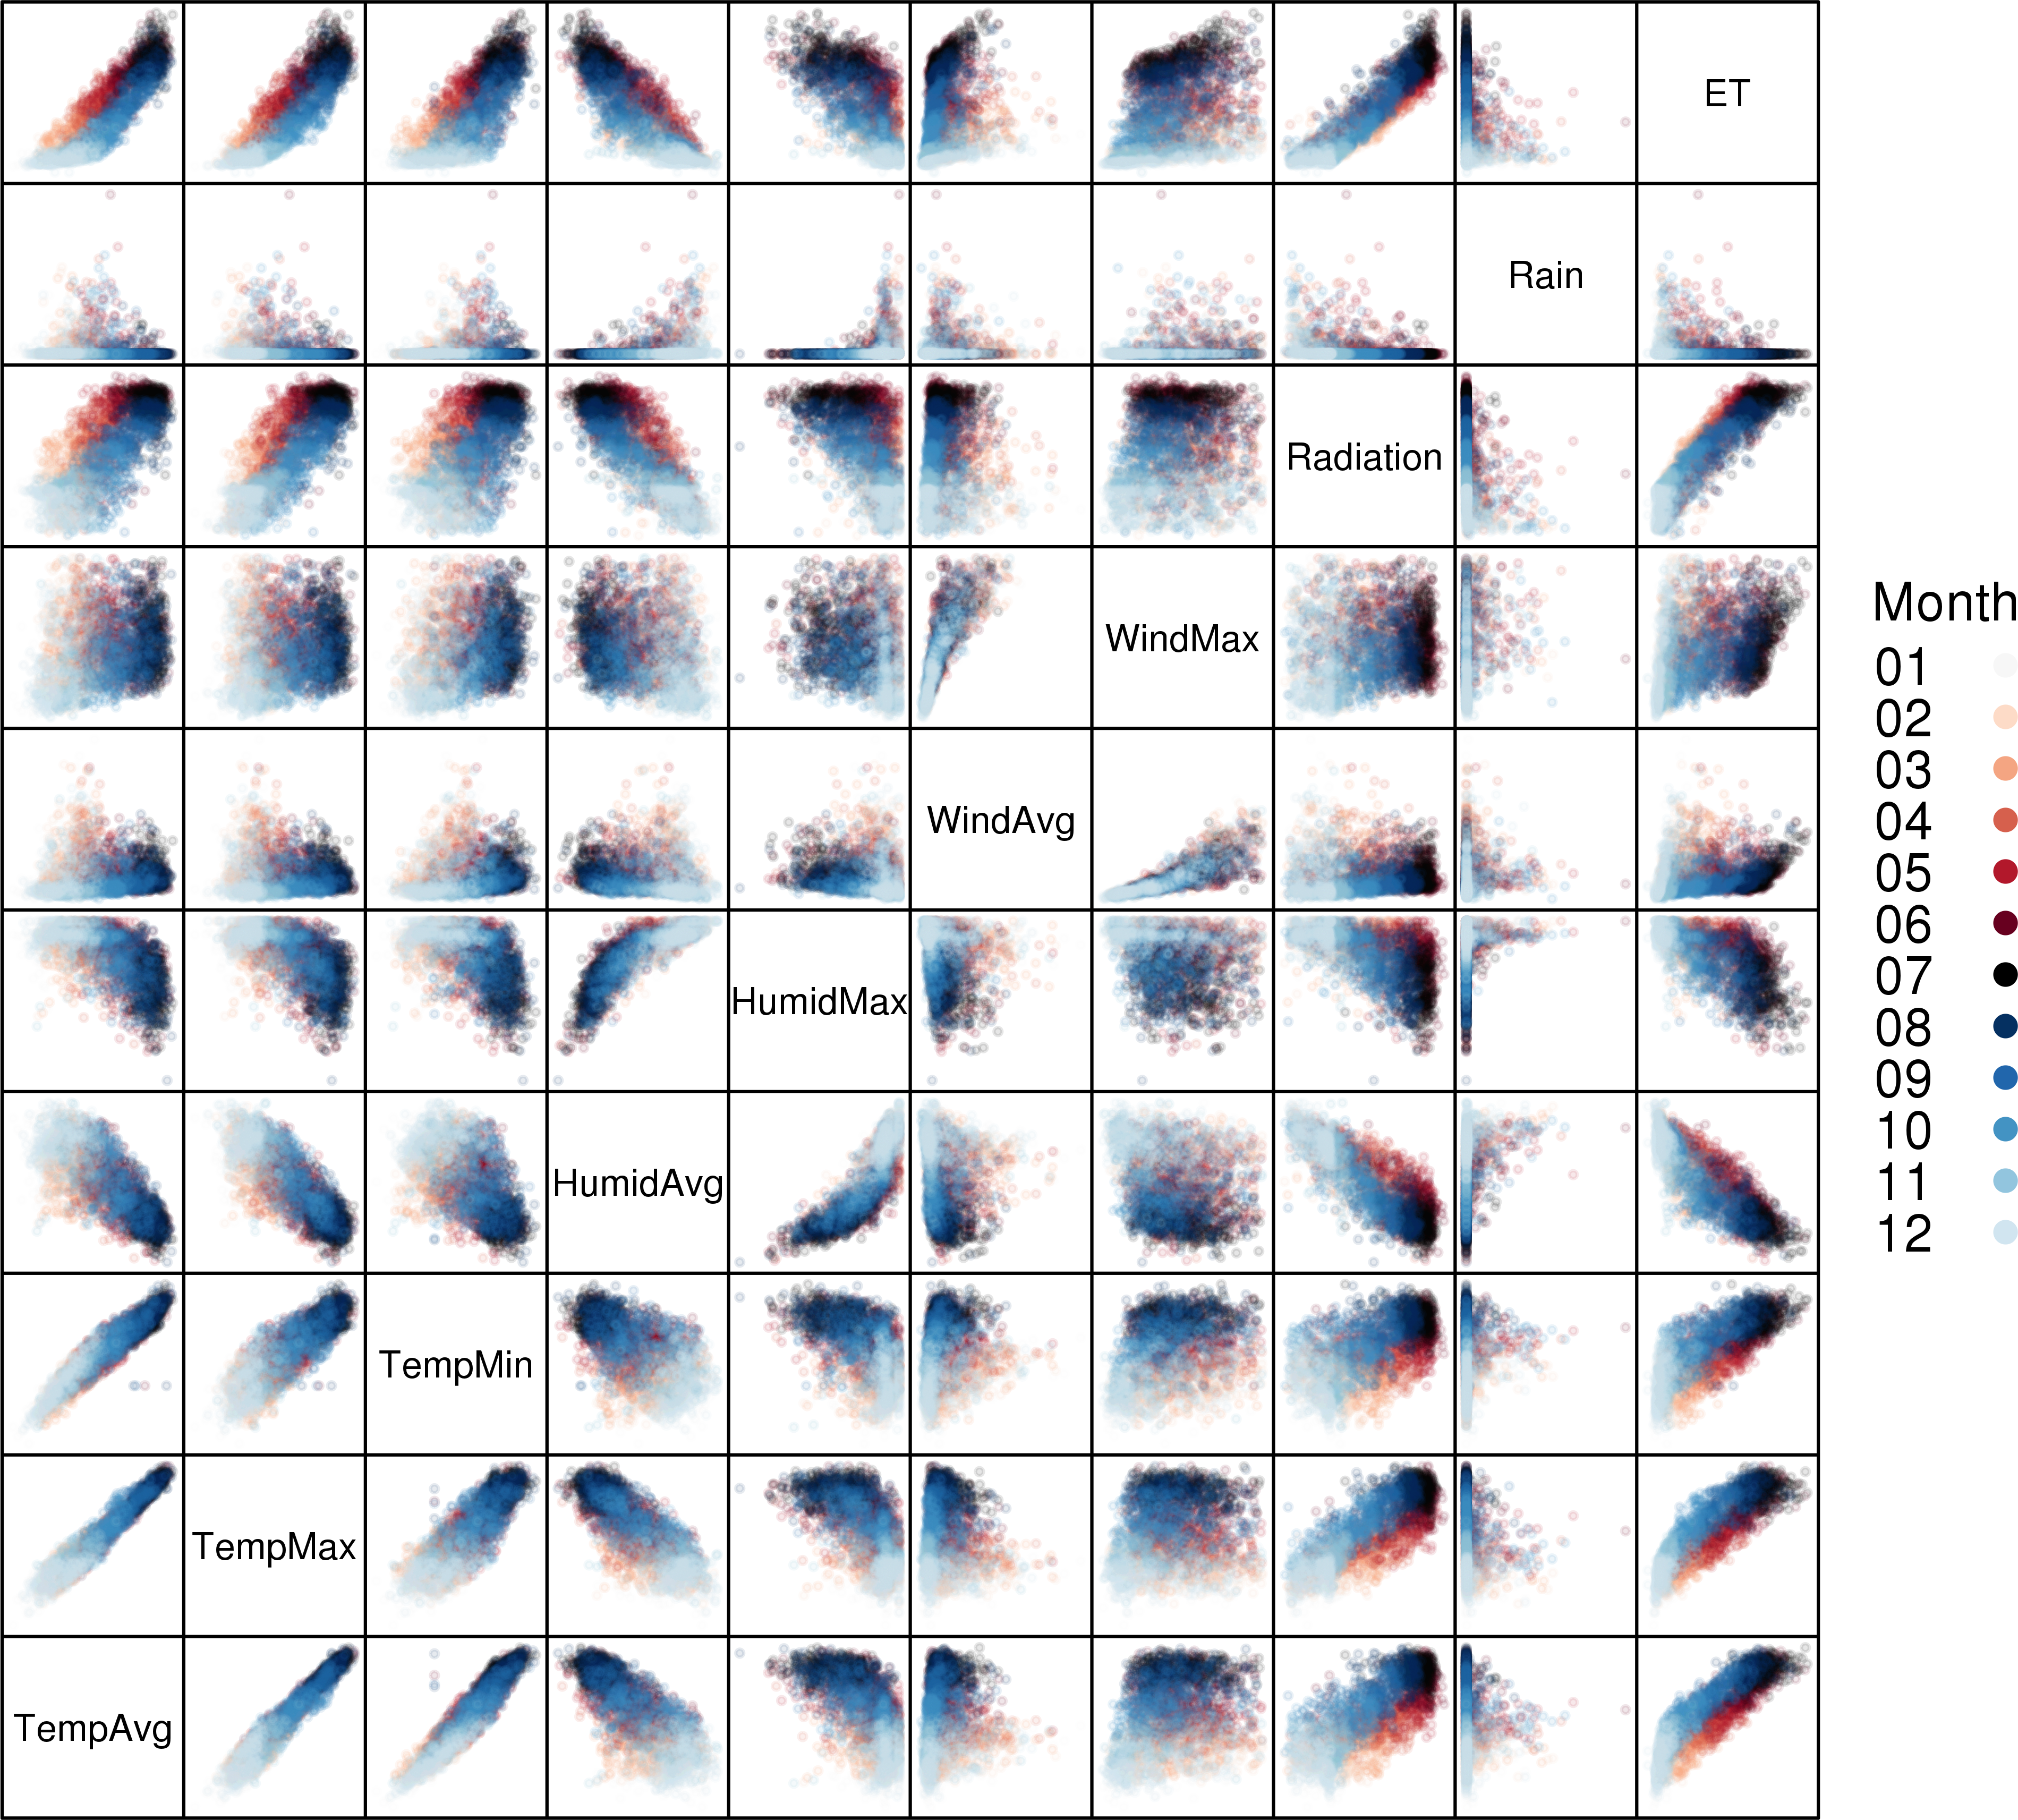
\includegraphics[width=.9\linewidth]{figs/aranjuezSplom.png}
\end{frame}




\subsection{Definir paneles con el índice temporal}
\label{sec-4-2}

\begin{frame}[fragile,label=sec-4-2-1]{ggplot2}
 \lstset{language=R,label= ,caption= ,numbers=none}
\begin{lstlisting}
  ggplot(data=aranjuezRshp,
         aes(Radiation, Temperature)) +
      facet_grid(Statistic ~ month) +
      geom_point(col='skyblue4',
                 pch=19, cex=0.5,
                 alpha=0.3) +
      geom_rug() +
      stat_smooth(se=FALSE, method='loess',
                  col='indianred1', lwd=1.2) +
      theme_bw()
\end{lstlisting}
\end{frame}

\begin{frame}[label=sec-4-2-2]{}
\includegraphics[width=.9\linewidth]{figs/aranjuezFacetGrid.png}
\end{frame}


\begin{frame}[fragile,label=sec-4-2-3]{lattice}
 \lstset{language=R,label= ,caption= ,numbers=none}
\begin{lstlisting}
  useOuterStrips(xyplot(Temperature ~ Radiation | month * Statistic,
                        data=aranjuezRshp,
                        between=list(x=0),
                        col='skyblue4', pch=19,
                        cex=0.5, alpha=0.3)) +
      layer({
          panel.rug(..., col.line='indianred1',
                    end=0.05, alpha=0.6)
          panel.loess(..., col='indianred1',
                      lwd=1.5, alpha=1)
      })
\end{lstlisting}
\end{frame}


\begin{frame}[label=sec-4-2-4]{}
\includegraphics[width=.9\linewidth]{figs/aranjuezOuterStrips.pdf}
\end{frame}


\section{Gráficos Interactivos}
\label{sec-5}
\subsection{googleVis}
\label{sec-5-1}

\begin{frame}[fragile,label=sec-5-1-1]{googleVis}
 \href{http://decastillo.github.io/googleVis_Tutorial/}{Tutorial}

\lstset{language=R,label= ,caption= ,numbers=none}
\begin{lstlisting}
library(googleVis)
\end{lstlisting}
\end{frame}

\begin{frame}[fragile,label=sec-5-1-2]{Ejemplo con datos de Navarra}
 \lstset{language=R,label= ,caption= ,numbers=none}
\begin{lstlisting}
navarraDF <- as.data.frame(navarra)
navarraDF <- stack(navarraDF)
navarraDF$ymd <- index(navarra)

navGVis <- gvisMotionChart(navarraDF,
                           idvar = 'ind', timevar='ymd')

plot(navGVis)
\end{lstlisting}
\end{frame}

\subsection{rCharts}
\label{sec-5-2}

\begin{frame}[fragile,label=sec-5-2-1]{rCharts}
 \url{http://ramnathv.github.io/rCharts/} 

\lstset{language=R,label= ,caption= ,numbers=none}
\begin{lstlisting}
library(rCharts)
\end{lstlisting}
\end{frame}

\begin{frame}[fragile,label=sec-5-2-2]{Highcharts}
 \url{http://www.highcharts.com/}

\lstset{language=R,label= ,caption= ,numbers=none}
\begin{lstlisting}
aranjuezDF <- as.data.frame(aranjuez)
## Highcharts necesita que las fechas sean numéricas
aranjuezDF$tt <-
    as.numeric(as.POSIXct(index(aranjuez)))*1000
hp <- hPlot(TempAvg ~ tt, data = aranjuezDF,
            type = 'line')
hp$xAxis(type = 'datetime')
hp
\end{lstlisting}
\end{frame}

\begin{frame}[fragile,label=sec-5-2-3]{Morris}
 \url{http://morrisjs.github.io/morris.js/}

\lstset{language=R,label= ,caption= ,numbers=none}
\begin{lstlisting}
mp <- mPlot(x = 'tt', y = c('TempAvg', 'TempMax'),
            data = aranjuezDF,
            type = 'Line')
## Ajustes para Morris            
mp$set(pointSize = 0, lineWidth = 1)
mp
\end{lstlisting}
\end{frame}

\begin{frame}[label=sec-5-2-4]{}

\end{frame}
% Emacs 24.3.1 (Org mode 8.2.7c)
\end{document}